
\textit{Calculus} means ``a method of calculation or reasoning.'' When one computes the sales tax on a purchase, one employs a simple calculus. When one finds the area of a polygonal shape by breaking it up into a set of triangles, one is using another calculus. Proving a theorem in geometry employs yet another calculus.

Despite the wonderful advances in mathematics that had taken place into the first half of the $17^\text{th}$ century, mathematicians and scientists were keenly aware of what they \textit{could not do.} (This is true even today.) In particular, two important concepts eluded mastery by the great thinkers of that time: area and rates of change. 

Area seems innocuous enough; areas of circles, rectangles, parallelograms, etc., are standard topics of study for students today just as they were then. However, the areas of \textit{arbitrary} shapes could not be computed, even if the boundary of the shape could be described exactly. 

Rates of change were also important. When an object moves at a constant rate of change, then ``distance = rate $\times $ time.'' But what if the rate is not constant -- can distance still be computed? Or, if distance is known, can we discover the rate of change?

It turns out that these two concepts were related. Two mathematicians, Sir Isaac Newton and Gottfried Leibniz, are credited with independently formulating a system of computing that solved the above problems and showed how they were connected. Their system of reasoning was ``a'' calculus. However, as the power and importance of their discovery took hold, it became known to many as ``the'' calculus. Today, we generally shorten this to discuss ``calculus.''

The foundation of ``the calculus'' is the \textit{limit.} It is a tool to describe a particular behavior of a function. This chapter begins our study of the limit by approximating its value graphically and numerically. After a formal definition of the limit, properties are established that make ``finding limits'' tractable. Once the limit is understood, then the problems of area and rates of change can be approached.

\section{The tangent problem}\label{sec:TangentProblem} %
Consider the computer- generated plot of the function $f(x)=\frac{x^2}2$ below. The line drawn in blue in Figure \ref{figTangentIdeaFor} appears to just touch the graph of the function $y=\frac{x^2}2$ at the point $P=(2,f(2))=(2, \frac{2^2}{2}) =(2,2)$. In mathematical language we say that the blue line is tangent to the graph of $ y=\frac{x^2}2$ (``tangent'' comes from Latin, ``to touch''). We shall give a formal definition of a tangent line later in Section \ref{secDefTangent}; until then, we shall refer to a ``tangent line'' informally, relying on the reader's intuition.

\begin{figure}[H]
	\centering
     \begin{tikzpicture}
     \begin{axis}[ %
     clip=false, 
     %minor x tick num=1,
     axis y line=middle,
     axis x line=middle,
     ymin=-1,
     ymax=5,
     %extra y tick labels={},
     xmin=-1,
     xmax=3.5,
     name=myplot]
     \addplot [{\colortwo},thick, smooth,domain=-1:3,samples=20] ({x},{x^2/2});
     \addplot [{\colorone},thick, smooth,domain=0.5:3,samples=20] ({x},{2*x-2});
     \coordinate (P) at (axis cs:2,2);
     %\coordinate (Q) at (axis cs:1.9,1.805);
     \end{axis}
     \node [right] at (myplot.right of origin) { $x$};
     \node [above] at (myplot.above origin) { $f$};
     %\draw [color=red, thick, shorten >= -1.9cm, shorten <=-1.9cm] (P)--(Q);
     \draw[color=\colorone,fill] (P) circle (0.1) node[above] {\scriptsize $P$} node[right] {\scriptsize $(2,2)$};
    % \draw[color=red,fill] (Q) circle (0.1)node[above] {\scriptsize $Q$} node[right] {\scriptsize $(1.9,1.805)$};     
     \end{tikzpicture} 
    \caption{   \label{figTangentIdeaFor} }
\end{figure}


We are seeking an equation for the tangent through $P=(2,2)=(2, f(2))$ drawn in \ref{figTangentIdeaFor}. We know one point on the tangent line - namely the point $P=(2,2)$. Recall that every non-vertical line has equation
\[
y=mx+c
\]
for some numbers $m$ and $c$, where $m$ is called the slope
of the line and $c$ is called the $y$-intercept of the line. As the tangent line passes through the point $P=(2,2)$, it has equation $y-2=m(x-2)$ for some slope $m$ that we yet need to define.

It is natural to approximate the tangent line using secant lines passing through the point $ P=(2, 2)$ and nearby points $Q=(t,f(t))=(t, \frac{t^2}{2})$ lying on the graph of $f(x)$. The line passing through $P=(2,2) $ and $Q=(t,f(t))$ has slope $m_{PQ}:=\frac{f(t)-2}{t-2}$ and therefore has equation
\[
y-2=m_{PQ}(x-2), \quad\quad \quad\text{where~} m_{PQ}= \left(\frac{f(t)-2}{t-2}\right).
\]
As the equation of the tangent line is $y-2=m(x-2)$, we choose to approximate $m$ by the numbers $m_{PQ}$ as $Q$ gets close to the point $P$. On the other hand, the point $Q=(t,f(t))$ gets closer to $P= (x, f(x))$ as $t$ gets closer to $x$.

\begin{figure}[H]
	\centering
	\begin{subfigure}[t]{0.33\textwidth}
		 \begin{tikzpicture}
		 \begin{axis}[ %
		 width=1.1\textwidth,
		 clip=false, 
		 %minor x tick num=1,
		 axis y line=middle,
		 axis x line=middle,
		 ymin=-1,
		 ymax=5,
		 %extra y tick labels={},
		 xmin=-1,
		 xmax=3.5,
		 name=myplot]
		 \addplot [{\colortwo},thick, smooth,domain=-1:3,samples=20] ({x},{x^2/2});
		 \coordinate (P) at (axis cs:2,2);
		 \coordinate (Q) at (axis cs:1,0.5);
		 \end{axis}
		 \node [right] at (myplot.right of origin) { $x$};
		 \node [above] at (myplot.above origin) { $f$};
		 \draw [color=\colorone, thick, shorten >= -1cm, shorten <=-1cm] (P)--(Q);
		 \draw[color=\colorone,fill] (P) circle (0.1) node[above] {\scriptsize $P$} node[right] {\scriptsize $(2,2)$};
		 \draw[color=\colorone,fill] (Q) circle (0.1)node[above] {\scriptsize $Q$} node[right] {\scriptsize $(1,1.5)$};
		 \end{tikzpicture}
        \label{ }
        \caption{$ t=1 $, $ m_{PQ}=1.5 $} 
    \end{subfigure}% 
 \begin{subfigure}[t]{0.33\textwidth}
     \begin{tikzpicture}
     \begin{axis}[ %
      width=1.1\textwidth,
     clip=false, 
     %minor x tick num=1,
     axis y line=middle,
     axis x line=middle,
     ymin=-1,
     ymax=5,
     %extra y tick labels={},
     xmin=-1,
     xmax=3.5,
     name=myplot]
     \addplot [{\colortwo},thick, smooth,domain=-1:3,samples=20] ({x},{x^2/2});
     \coordinate (P) at (axis cs:2,2);
     \coordinate (Q) at (axis cs:1.5,1.125);
     \end{axis}
     \node [right] at (myplot.right of origin) { $x$};
     \node [above] at (myplot.above origin) { $f$};
     \draw [color=\colorone, thick, shorten >= -1.5cm, shorten <=-1.5cm] (P)--(Q);
      \draw[color=\colorone,fill] (P) circle (0.1) node[left] {\scriptsize $P$} node[right] {\scriptsize $(2,2)$};
      \draw[color=\colorone,fill] (Q) circle (0.1)node[left] {\scriptsize $Q$} node[right] {\scriptsize $(1.5,1.125)$};
     \end{tikzpicture} %
        \label{ }
        \caption{$ t=1.5 $, $ m_{PQ}=1.75 $} 
    \end{subfigure}
 \begin{subfigure}[t]{0.33\textwidth}
     \begin{tikzpicture}
     \begin{axis}[ %
      width=1.1\textwidth,
     clip=false, 
     %minor x tick num=1,
     axis y line=middle,
     axis x line=middle,
     ymin=-1,
     ymax=5,
     %extra y tick labels={},
     xmin=-1,
     xmax=3.5,
     name=myplot]
     \addplot [{\colortwo},thick, smooth,domain=-1:3,samples=20] ({x},{x^2/2});
     \coordinate (P) at (axis cs:2,2);
     \coordinate (Q) at (axis cs:1.9,1.805);
     \end{axis}
     \node [right] at (myplot.right of origin) { $x$};
     \node [above] at (myplot.above origin) { $f$};
     \draw [color=\colorone, thick, shorten >= -1.9cm, shorten <=-1.9cm] (P)--(Q);
     		 \draw[color=\colorone,fill] (P) circle (0.1) node[above] {\scriptsize $P$} node[right] {\scriptsize $(2,2)$};
     		 \draw[color=\colorone,fill] (Q) circle (0.1)node[left] {\scriptsize $Q$} node[below right] {\scriptsize $(1.9,1.805)$};     
     \end{tikzpicture}
        \label{ }
      \caption{$ t=1.9 $, $ m_{PQ}=1.95 $}  
    \end{subfigure} 
    \caption{ Slopes of secant lines as $ Q $ approaches $ P $ from the left.  \label{tangentleft} }
\end{figure}


\begin{figure}[H]
	\centering
	\begin{subfigure}[t]{0.33\textwidth}
		 \begin{tikzpicture}
		 \begin{axis}[ %
		 width=1.1\textwidth,
		 clip=false, 
		 %minor x tick num=1,
		 axis y line=middle,
		 axis x line=middle,
		 ymin=-1,
		 ymax=5,
		 %extra y tick labels={},
		 xmin=-1,
		 xmax=3.5,
		 name=myplot]
		 \addplot [{\colortwo},thick, smooth,domain=-1:3,samples=20] ({x},{x^2/2});
		 \coordinate (P) at (axis cs:2,2);
		 \coordinate (Q) at (axis cs:3,4.5);
		 \end{axis}
		 \node [right] at (myplot.right of origin) { $x$};
		 \node [above] at (myplot.above origin) { $f$};
		 \draw [color=\colorone, thick, shorten >= -1cm, shorten <=-1cm] (P)--(Q);
		 \draw[color=\colorone,fill] (P) circle (0.1) node[left] {\scriptsize $P$} node[below right] {\scriptsize $(2,2)$};
		 \draw[color=\colorone,fill] (Q) circle (0.1)node[above left] {\scriptsize $Q$} node[right] {\scriptsize $(3,4.5)$};
		 \end{tikzpicture}
        \label{ }
        \caption{$ t=3 $, $ m_{PQ}=2.5 $} 
    \end{subfigure}% 
 \begin{subfigure}[t]{0.33\textwidth}
     \begin{tikzpicture}
     \begin{axis}[ %
      width=1.1\textwidth,
     clip=false, 
     %minor x tick num=1,
     axis y line=middle,
     axis x line=middle,
     ymin=-1,
     ymax=5,
     %extra y tick labels={},
     xmin=-1,
     xmax=3.5,
     name=myplot]
     \addplot [{\colortwo},thick, smooth,domain=-1:3,samples=20] ({x},{x^2/2});
     \coordinate (P) at (axis cs:2,2);
     \coordinate (Q) at (axis cs:2.5,3.125);
     \end{axis}
     \node [right] at (myplot.right of origin) { $x$};
     \node [above] at (myplot.above origin) { $f$};
     \draw [color=\colorone, thick, shorten >= -1.5cm, shorten <=-1.5cm] (P)--(Q);
      \draw[color=\colorone,fill] (P) circle (0.1) node[left] {\scriptsize $P$} node[below right] {\scriptsize $(2,2)$};
      \draw[color=\colorone,fill] (Q) circle (0.1)node[above left] {\scriptsize $Q$} node[right] {\scriptsize $(2.5,3.125)$};
     \end{tikzpicture} %
        \label{ }
        \caption{$ t=2.5 $, $ m_{PQ}=2.25 $} 
    \end{subfigure}
 \begin{subfigure}[t]{0.33\textwidth}
     \begin{tikzpicture}
     \begin{axis}[ %
      width=1.1\textwidth,
     clip=false, 
     %minor x tick num=1,
     axis y line=middle,
     axis x line=middle,
     ymin=-1,
     ymax=5,
     %extra y tick labels={},
     xmin=-1,
     xmax=3.5,
     name=myplot]
     \addplot [{\colortwo},thick, smooth,domain=-1:3,samples=20] ({x},{x^2/2});
     \coordinate (P) at (axis cs:2,2);
     \coordinate (Q) at (axis cs:2.1,2.205);
     \end{axis}
     \node [right] at (myplot.right of origin) { $x$};
     \node [above] at (myplot.above origin) { $f$};
     \draw [color=\colorone, thick, shorten >= -1.9cm, shorten <=-1.9cm] (P)--(Q);
     		 \draw[color=\colorone,fill] (P) circle (0.1) node[left] {\scriptsize $P$} node[below right] {\scriptsize $(2,2)$};
     		 \draw[color=\colorone,fill] (Q) circle (0.1)node[above left] {\scriptsize $Q$} node[right] {\scriptsize $(2.1,2.205)$};     
     \end{tikzpicture}
        \label{ }
      \caption{$ t=2.1 $, $ m_{PQ}=2.05 $}  
    \end{subfigure} 
    \caption{ Slopes of secant lines as $ Q $ approaches $ P $ from the right.  \label{tangentright} }
\end{figure}






In Table \ref{tableTangentIdeaForTable}, we have computed the values of $f(t)$ and $m_{PQ}=\frac{f(t)-2}{t-2}$ for various values of $t$ close to $x=2$.  In Figures \ref{tangentleft}-\ref{tangentright}, and in Table \ref{tableTangentIdeaForTable} we see that as $t$ gets closer to $2$, $m_{PQ}$ appear to get closer to the number $2$, and indeed, we can say that $m_{PQ}$ ``gets infinitely close to $2$ as $t$ approaches $2$'' and so we can define $m=2$. Then the equation of the equation of the tangent line at $P$ becomes
\[
y-2=2(x-2)\quad ,
\]
which is exactly the equation of the line plotted in blue in Figure \ref{figTangentIdeaFor}.

\mTable{1}{Values of $f(x)$ and slope of line through $P,Q$.}{tableTangentIdeaForTable}{\begin{tabular}{c|c|c|c|c}
$x$& $f(x)=\frac{t^2}2$& $t-2$ & $f(t)-f(2)$ & $m_{PQ}=\frac{f(t)-f(2)}{t-2}$ \\\hline
0& 0& -2& -2& 1 \\
1& 0.5& -1& -1.5& 1.5 \\
1.5& 1.125& -0.5& -0.875& 1.75\\
1.9& 1.805& -0.1& -0.195& 1.95\\
1.99& 1.98005& -0.01& -0.01995& 1.995\\
1.999& 1.998& -0.001& -0.0019995& 1.9995\\\hline
2.001& 2.002& 0.001& 0.0020005& 2.0005\\
2.01& 2.02005& 0.01& 0.02005& 2.005\\
2.1& 2.205& 0.1& 0.205& 2.05\\
2.5& 3.125& 0.5& 1.125& 2.25\\
3& 4.5& 1& 2.5& 2.5\\
4& 8& 2& 6& 3 \\
\end{tabular}}


In order to give a strict definition of tangent, we need to define formally what it means for $m_{PQ}$ to ``get infinitely close'' to the number $2$. The colloquial phrase ``to get infinitely close to,'' corresponds to the mathematical notion of taking limits.

\subsection*{Velocity:}

A similar idea is behind our notion of \textit{velocity}. We can see immediately
how fast we are going, that is we can find the \textit{instantaneous velocity} of a
car we are driving just by looking at the speedometer. But what is that actually
measuring? The \textit{average velocity} makes sense, it's the distance travelled
over a specific interval of time. But the speedometer doesn't measure that, it
has a reading at each instant, and does not calculate an average velocity.

But the idea of instantaneous velocity of a moving car, at a specific time,
has to be interpreted as another limiting process, taking average velocities
over shorter and shorter time intervals:\[
velocity\, \, v:=\lim _{\Delta t\rightarrow 0}\frac{\Delta distance}{\Delta t}\]
where \( \Delta t \) means {}``the change in time{}'', \( \Delta =change\, in \).

If you plot the distance on the vertical axis, and time on the horizontal, then
you have the same picture as before, and the velocity is the slope of that graph. 


%In the following exercises, we continue our introduction and approximate the value of limits.\\
%
%\printexercises{exercises/01_01_exercises}


%One-sides:
%
%\printexercises{exercises/01_04_exercises}


%%%%%%%%%%%%%%%%%%%%%%%%%%%%%%%%%%%%%%%%%%%%
\Opensolutionfile{solutions}[ex]
\section*{Exercises for Section \ref{sec:TangentProblem}}

\begin{multicols}{2}

\begin{enumialphparenastyle}

%%%%%%%%%%
% % % % % % % % % % %
\begin{ex}
Estimate the slope of the tangent line to the curve $f(x)=2\sin\frac{x}{2}$ at
the point $(\frac{\pi}{2},\sqrt{2})$.
 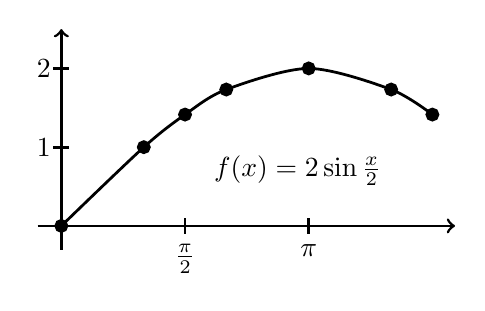
\begin{tikzpicture}[line width=1pt,scale=1]
\draw[->] (0,-.3) -- (0,2.5);
\foreach \x in {1,2} 
{\draw (-.1,\x) --node[left]{\x} (.1,\x);
}
\draw[->] (-.3,0) -- (5,0);
\foreach \x in {2,4} 
{\draw (\x*pi/4,-.1) -- (\x*pi/4,.1);
}
\draw node[below=.1cm] at (pi/2,0) {$\frac{\pi}{2}$};
\draw node[below=.1cm] at (pi,0) {$\pi$};
\draw plot[smooth,mark=*] coordinates{(0,0) (pi/3,1) (pi/2,1.414) (2*pi/3,1.732)
(pi,2) (4*pi/3,1.732) (3*pi/2,1.414)};
\draw node  at (3,.7) {$f(x)=2\sin\frac{x}{2}$};
\end{tikzpicture}
\end{ex}



\begin{ex}
The following graphic shows 5 students and their grades posted compared to the
number of cookies that they made for me. Estimate the G.P.A. of a student who
makes me 17 cookies.
\[
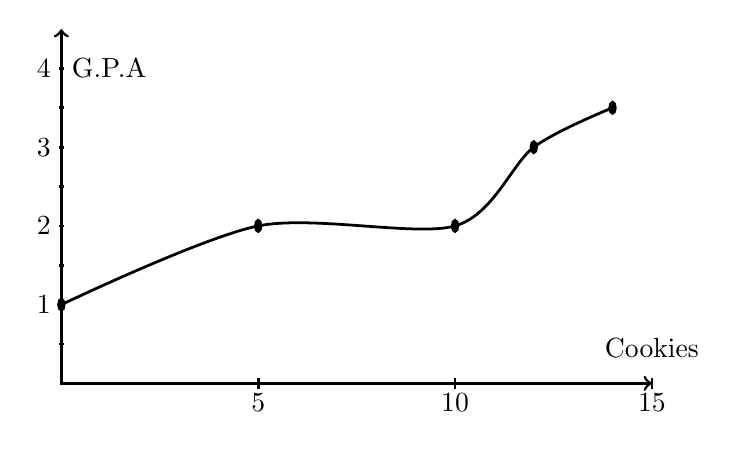
\begin{tikzpicture}[line width=1pt,xscale=.5]
\draw[<->] (0,4.5) -- (0,0) -- (15,0);
\foreach \x in {.5,1,...,4} \draw (-.07,\x) -- (.07,\x);
\foreach \x in {1,2,3,4} \draw node[left] at (0,\x) {$\x$};
\draw node[right] at (0,4) {G.P.A};
\foreach \x in {5,10,15} 
{
\draw (\x,-.07) -- (\x,.07);
\draw node[below] at (\x,0) {$\x$};
}
\draw node[above] at (15,0.2) {Cookies};
\draw plot[smooth,mark=*] coordinates{(0,1) (5,2) (10,2) (12,3) (14,3.5)};
\end{tikzpicture}
\]
\end{ex}


\begin{ex}
 Gravity on Earth dictates that a projectile with initial velocity of $v_0$ and starting height of $h_0$ has height (in feet) at time $t$ given by 
\[
 h(t)=-16t^2+v_0t+h_0.
\]
A rock dropped off the Twin Falls bridge takes $ 6 $ seconds to reach the river below. Find the average velocity of the rock.
\end{ex}


\begin{ex}
  If a rock is thrown upward on the planet Oz with a velocity of $ 20 $ m/s, its height in meters $t$ seconds later is given by $y=20t-10t^2$. Find the average velocity over the given time intervals:
\begin{itemize} 
    \item $[1,2]$
    \item $[1,1.5]$
    \item $[1,1.1]$
    \item $[1,1.01]$
\end{itemize}
  Estimate the instantaneous velocity when $t=1$.
\end{ex}

\end{enumialphparenastyle}

\end{multicols}